	
\documentclass[11pt]{article}


%\usepackage{url}
\usepackage{latexsym}
\usepackage{hyperref} 
\usepackage{graphicx}
\usepackage{verbatim}
\usepackage{geometry}

\begin{document}

%\pagenumbering{gobble}

%\begin{figure}[t]
%\includegraphics[width=4cm]{KCLlogo}
%\centering
%\end{figure}


\title{\textbf{7CCSMGPR Group Project}
\textbf{Initial Report} \textbf{Traffic Simulator Engine}}

%\author{\textbf{Authors:}\\ 
%Awasthi Saumya, Czapski Fabian Sebastian, \\
%Gangwani Dhiraj, Mohan Naveena, Serna Silva Lorena}

%\maketitle


%\renewcommand\contentsname{Table of Contents}
%\tableofcontents
%\phantomsection


%\pagenumbering{arabic}
%\setcounter{page}{3}

\begin{center}
\underline{ \textbf{7CCSMGPR Group Project: Traffic Simulator Engine} }
\end{center}

\section{Project Description}\label{PD}
	
	\subsection{Project Aims}\label{Aims}
	The aim of this project is to create a traffic simulation engine, allowing users i.e. Traffic Engineers to configure the following input configurations to demonstrate and generate reports for various traffic behaviours:\\
	%\begin{itemize}
		$\bullet$ To build any kind of road network with customized parameters.\\
		$\bullet$ Configurable traffic pattern options contributed by different vehicle types, traffic density, traffic lights synchronization, driver behaviour, climatic conditions, etc.
	%\end{itemize}
		

	\subsection{Strategy}\label{Strat}
		\underline{ \textit{Evaluation of Approaches:}} Evaluation of various approaches which could be adopted for the development of the simulation engine in Java were considered:\\
		 $\bullet$ An agent driven approach with 3rd party extension and library, like Repast and JADE.\\
		 $\bullet$ An object oriented approach which involves identifying all elements and interactions as objects as well as their behaviours, programming everything from scratch was adopted. 
	\\
	\underline { \textit{Analysis of the Requirements:} }
	Since the existing given requirements were generic, the team revisited and redefined them to create the formal specification document.  \\
	\underline { \textit{Software Design and Architecture:}} The problem is approached using the following architectural methodologies and patterns in software design and development:
	\\ $\bullet$ Decomposition of the problem and definition of the use case as shown in Fig. \ref{fig:HLD}. \\
		$\bullet$ Identification of various components in the ecosystem, their interactions and dependencies with UML 2 as can be seen in the following Fig. \ref{fig:FCD}.\\
		$\bullet$ Identification of the attributes and methods of each sub component using ArgoUML.\\
		$\bullet$ Grouping related components into controllers and developing Interface Contracts with method signatures for the interactions between User Interface and Simulation Engine.\\
	%\end{itemize}
	\underline {\textit{Software Development, Testing and Documentation:}} Agile software development methodology is adopted. The team is divided into two sub teams namely the UI (Front End) Team and Engine Team (Back End), each of them focusing on one of the two major components at the high level architecture, Fig. \ref{fig:HLD}. Each team identifies their major tasks and subtasks to ensure cross team and parallel implementation. A Sprint model will be followed with regular status updates in Scrum meetings for tasks identification, allocation, development, testing, bug fixes and documentation of each Sprint.


	\subsection{Timetable}\label{TT}
	Each Sprint has been identified with tasks for both teams with emphasis on accomplishing the aims and if time permits, secondary aims would be accomplished as well. 
		\begin{figure}[h]
		     	\centering
    			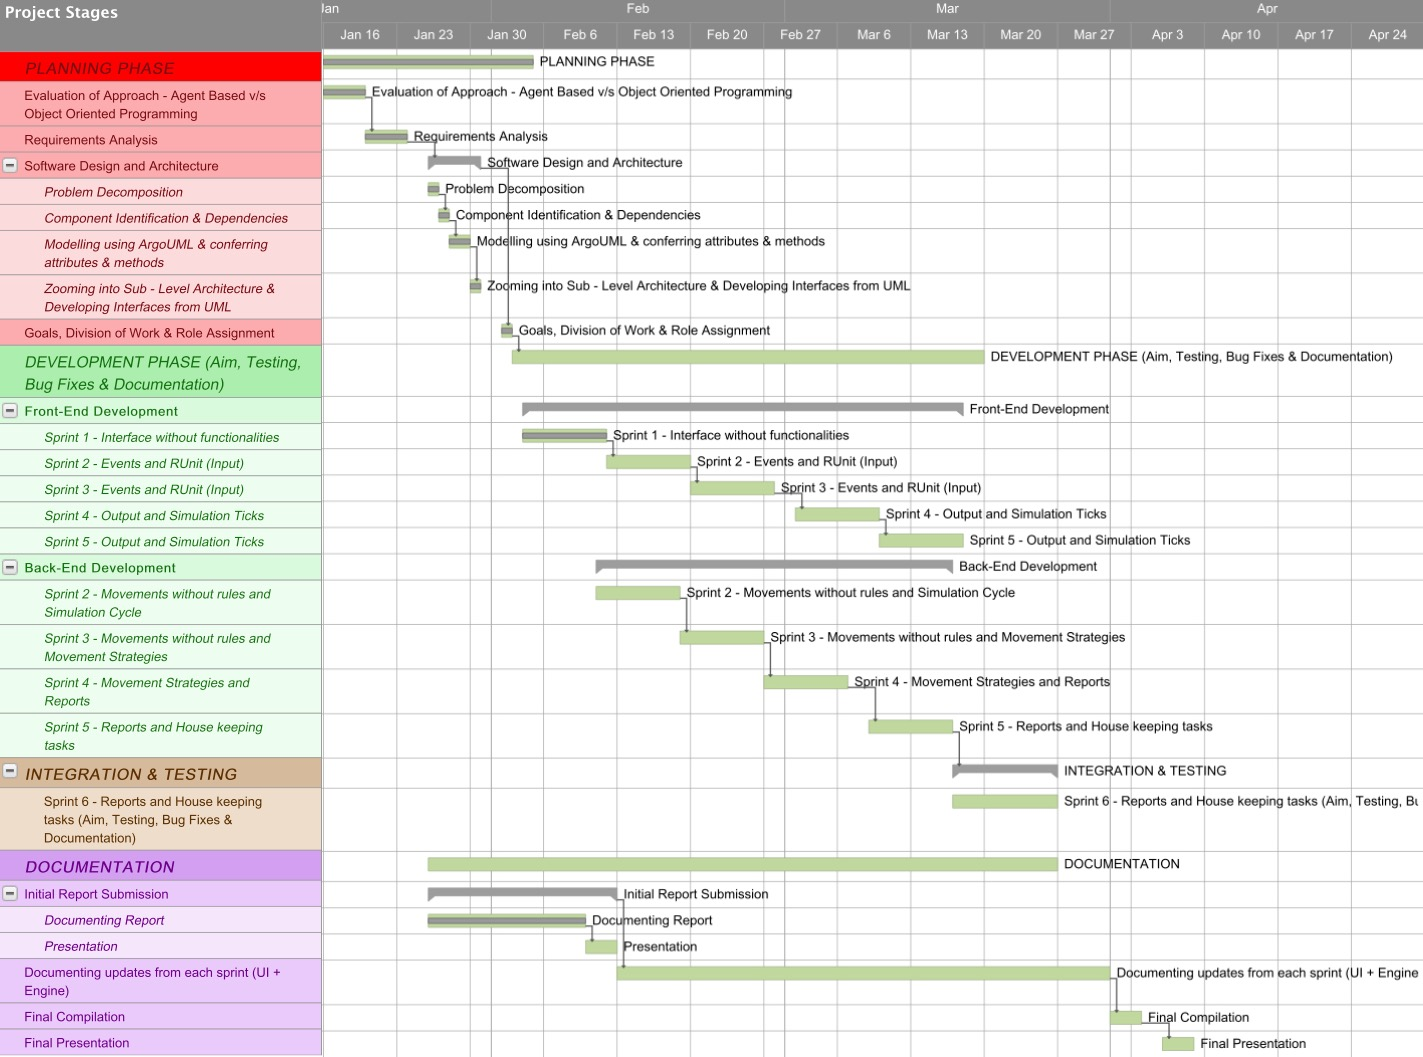
\includegraphics[width=0.6\textwidth]{Gantt}
    			\caption{Gantt Chart}
    			\label{fig:GC}
		\end{figure}
	\\
	\underline { \textit{Primary Aims} } \\
	%\begin{itemize} 
		$\bullet$ Uploading of a road network background image (e.g. a Google Map snapshot) or whiteboard on which the user can draw, configure the road network and infrastructure.\\
		$\bullet$ User configurable road networks with traffic elements, traffic light cycles, driver characteristics, weather conditions, and emergency vehicle routing.\\
		$\bullet$  Implementation of basic driver and vehicle behaviour.\\
	 	$\bullet$ Generation of reports for various traffic management policies.
	%\end{itemize}
	\\
	\underline { \textit{Secondary Aims} }
	\\
	%\begin{itemize} 
		$\bullet$ User configurable destination based routing.\\
		 $\bullet$ Importing/exporting of road network and infrastructure configuration using a CSV file.\\
		 $\bullet$ Advanced driver behaviour such as congestion avoidance.
	%\end{itemize}

	\subsection{Progress Achieved and Current Status}\label{PACS}
	%\begin{itemize}
		 $\bullet$ Adopted the object oriented approach after evaluating other options.\\
		 $\bullet$ Analysed the requirements and formalized the requirement specification.\\
		 $\bullet$ Designed the high level architecture by identifying the two main components. Fig. \ref{fig:HLD}.\\
		%\begin{itemize}
		\hspace*{1.5ex} $\circ$ \textit{User Interface} will allow the user to create the road network and interact with it by playing the simulation as well as generating reports.\\
		\hspace*{1.5ex} $\circ$ \textit{Simulation Engine} will move the vehicles on the configured roads and based on the other configured parameters including the change of lights.
			\begin{figure}[h]
		     		\centering
    				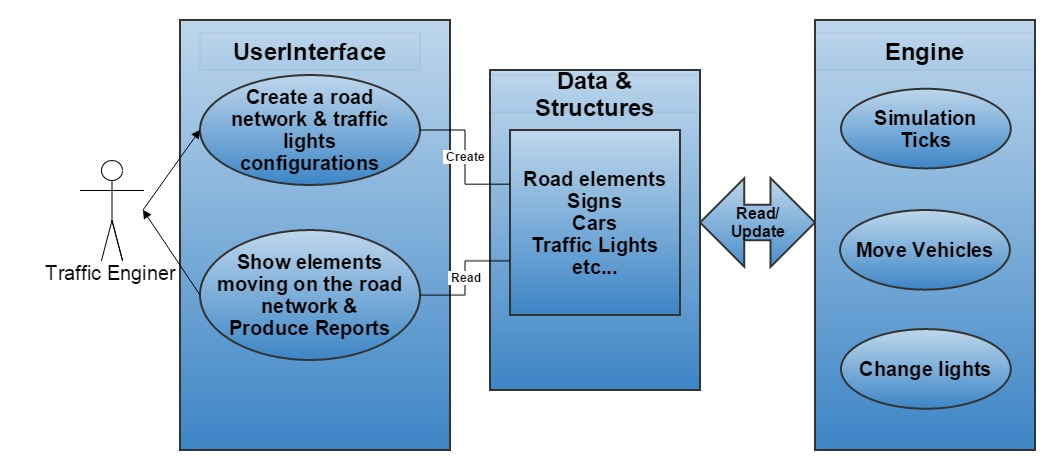
\includegraphics[width=0.7\textwidth]{highlevel}
    				\caption{Problem Decomposition and Use Case Definition}
    				\label{fig:HLD}
			\end{figure}
		%\end{itemize}
		\\
		 $\bullet$ Designed the main system components as Interfaces, their interactions and dependencies, Fig. \ref{fig:FCD}. Identified other interfaces and individual classes in sub components and populated the attributes and methods. 
			\begin{figure}[h]
			     \centering
    				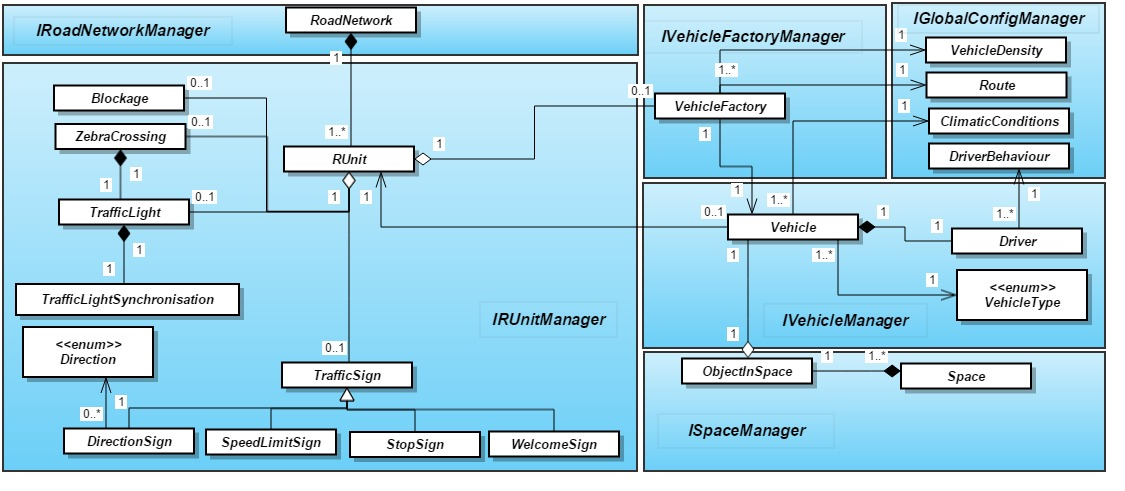
\includegraphics[width=0.9\textwidth]{fullclassdiagram}
    				\caption{Component Identification and Interactions using UML 2}
    				\label{fig:FCD}
			\end{figure}	
		\\
		 $\bullet$ Developed Interface Contracts with method signatures for the interactions between User Interface and Simulation Engine.\\
		 $\bullet$ Ongoing development of the UI.
	%\end{itemize}


\section{Project Organisation}\label{Section-PO}

		\subsection{Team Work Plan}\label{SubSec-TWP} The approach of Agile development was adopted. This facilitates collaboration between sub teams within the group namely the User Interface (UI Team) and Engine Team. During the group meetings, the sub teams narrowed down on their main tasks and accordingly divided them amongst the members, assigning roles to every member.

		\subsection{Roles Played by Members}\label{SubSec-RPM} 
		 $\bullet$ Project Coordinator: Naveena Mohan\\
		 $\bullet$ Software Architect: Fabian Czapski\\
		 $\bullet$ Quality Assurance: Dhiraj Gangwani\\
		 $\bullet$ Documentation Manager: Lorena Serna\\
		 $\bullet$ UI Developers: Saumya Awasthi, Naveena Mohan, Dhiraj Gangwani\\
		 $\bullet$ Engine Developers: Lorena Serna, Fabian Czapski
			

		\subsection{Tools Used for Collaboration}\label{SubSec-TUC}
		%\begin{itemize}
		 $\bullet$ Design and Architecture $\rightarrow$ Argo UML\\
		 $\bullet$ Development and Testing $\rightarrow$ IntelliJ and Eclipse\\
		 $\bullet$ Project Management $\rightarrow$ Freed Camp\\
		 $\bullet$ Version Control $\rightarrow$ Git\\
		 $\bullet$ Documentation Repository $\rightarrow$ Google Sites\\
		 $\bullet$ Documentation Report $\rightarrow$ Latex\\
		 $\bullet$ Communication $\rightarrow$ Facebook Group  and WhatsApp Messenger
		%\end{itemize}

		\subsection{Peer Assessment}\label{SubSec-PA} A total of 100 points would be equally split among the five team members anonymously where each team member would allocate their twenty points to the other four members based on their performance (excluding himself/herself). Points an individual team member allocates to the others must sum up to twenty. \\
Advantage of this approach is that the peer assessment can be anonymous and unbiased. However this approach has a drawback where the members from a sub team would be unaware of the contributions of the members in other team at a certain stage in the project. This would be taken care in the regular status updates in the Scrum meetings.

		\subsection{Team Conflict Management}\label{SubSec-TCM} Conflicts are going to be handled maturely and sportingly in the event of absence of a team member during team meetings and/or accomplishing the task deadlines. Below are certain instances of probable conflicts and their possible resolutions: \\
		%\begin{itemize}
		      $\bullet$ It is an individual\rq s responsibility to update themselves with the discussions during the meeting and the tasks assigned to them. \\
			$\bullet$ On encountering disagreements during meetings and brainstorming sessions, an unbiased opinion of all team members will be taken into consideration. The most suitable opinion, beneficial for the project will be finalized. \\
		 	$\bullet$ Failure on meeting a task deadline in a particular Sprint by a team member should be handled with high priority in the upcoming sprint tasks. 
		%\end{itemize}

\bibliography{reference}
\bibliographystyle{plain}

\end{document}
